\section{Empirical application: calibrated virtual sensing of daily PM$_{2.5}$ in the Po Valley}
\label{sec:po_application}

\subsection{Application objective and locked external-test design}
\label{subsec:po_design}

The empirical study evaluates daily PM$_{2.5}$ virtual sensing at monitoring sites that are completely unseen during model development. The task is spatial prediction rather than ahead-of-time forecasting: on each target day, PM$_{2.5}$ observations from the active development network are available, whereas the PM$_{2.5}$ value at the target site is treated as unobserved. Meteorological variables and static site attributes are available at both source and target locations. This setting represents temporary sensor failure, expansion of a monitoring network, or retrospective exposure reconstruction at a location without an operating PM$_{2.5}$ instrument.

The data set contains daily observations from 50 stations during 2018--2023. Forty stations were assigned to model development and ten stations were locked before any final evaluation. The development protocol used 2018--2021 for mean-model fitting and 2022 for whole-station validation, early stopping, uncertainty estimation, and conformal calibration. After the complete modeling pipeline had been fixed, it was applied once to the ten locked stations in 2023. No PM$_{2.5}$ observation from a locked station was used to estimate the station climatology, train the daily anomaly model, learn graph weights, fit the Student-$t$ scale model, or determine the conformal factor.

The locked test comprised 3,237 station--day observations from 359 calendar days. Six target stations were background sites, three were traffic sites, and one was industrial; seven were urban and three suburban. The nearest development station was between 2.52 and 28.99~km away, with a median distance of 17.35~km. Across the locked observations, mean PM$_{2.5}$ was 17.35~$\mu\mathrm{g}\,\mathrm{m}^{-3}$, the median was 13.97, the 90th percentile was 34.00, and the maximum was 203.00. Figure~\ref{fig:po_station_design} shows the spatial separation between the development network and the locked external-test sites.

\begin{figure}[htbp]
    \centering
    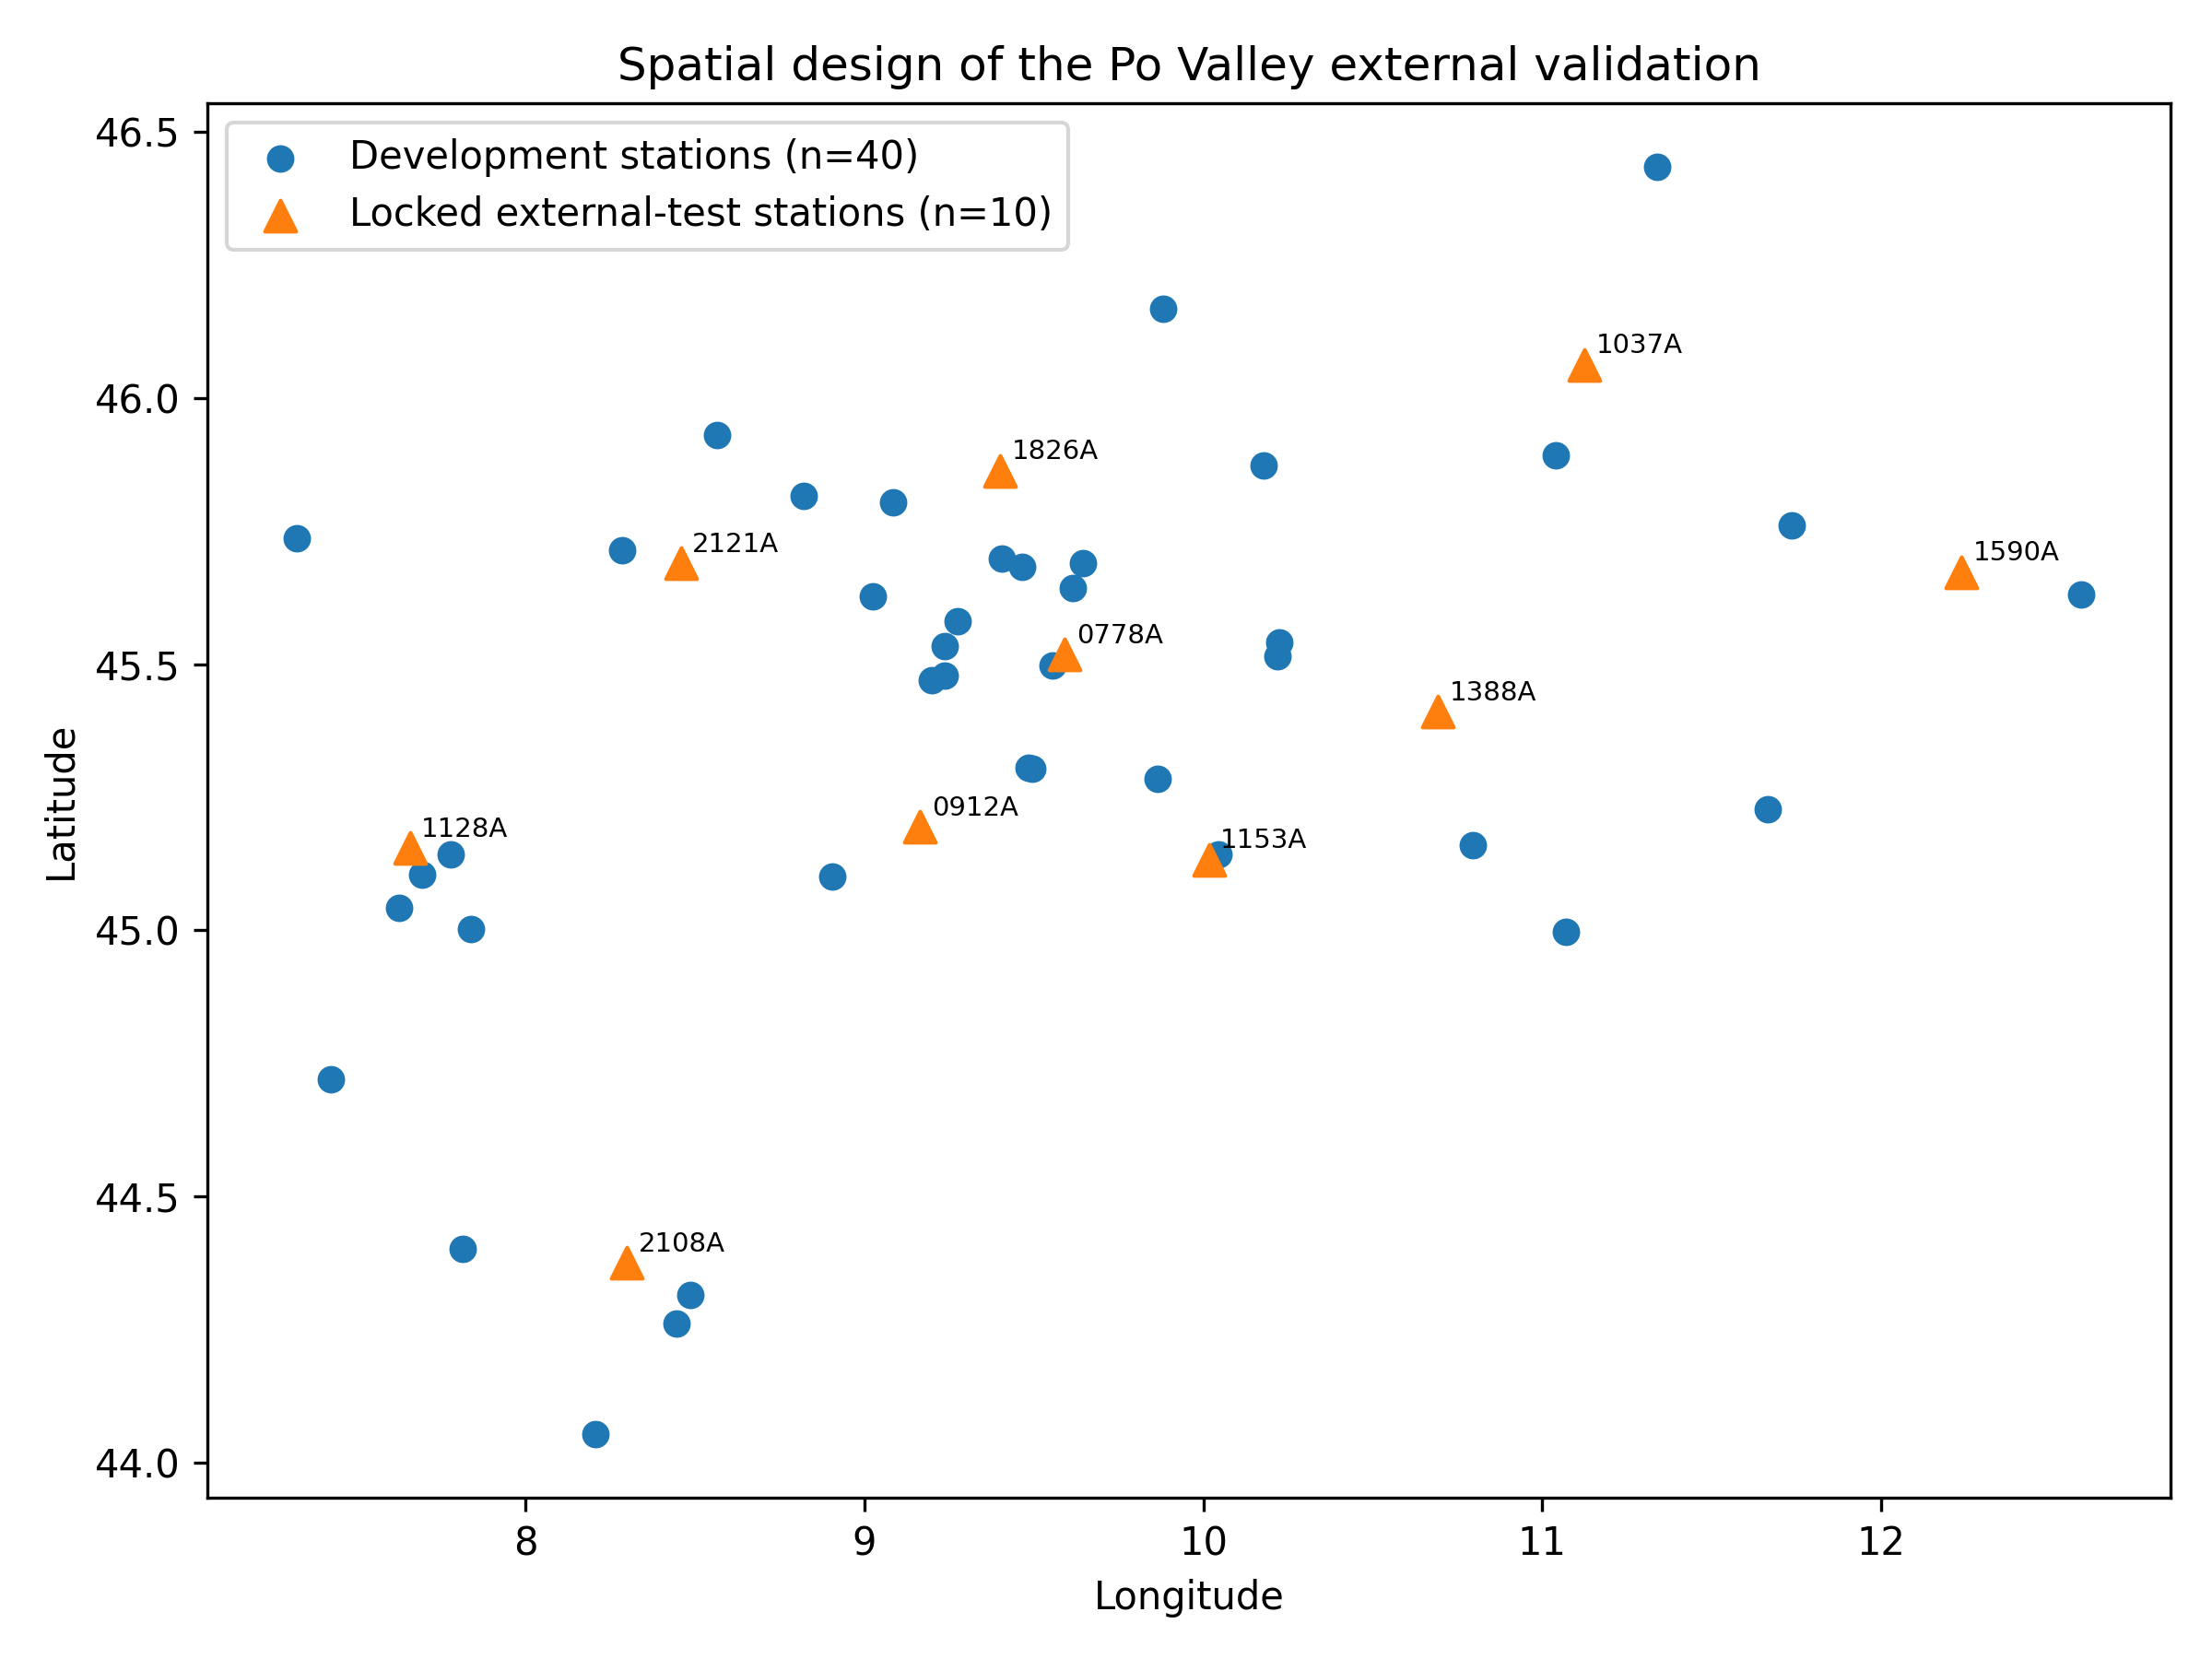
\includegraphics[width=0.86\linewidth]{figures/fig_po_station_design.png}
    \caption{Spatial design of the external validation. Circles indicate the 40 development stations and triangles indicate the ten monitoring sites locked before final evaluation. Numeric labels identify the locked stations.}
    \label{fig:po_station_design}
\end{figure}

\subsection{Frozen deployment pipeline}
\label{subsec:po_frozen_model}

The frozen pipeline contains four components. First, a regularized kernel model estimates the long-run station climatology from coordinates, altitude, station type, area class, and the 2018--2021 meteorological climatology. Source-station climatologies are generated by leave-one-station-out fitting, so their training representation mimics application at a site with no PM$_{2.5}$ history. The climatology of each locked station is then estimated from all 40 development stations.

Second, a gradient-boosted daily anomaly model predicts deviations from the station climatology using boundary-layer height, relative humidity, temperature, precipitation, wind speed, solar radiation, vegetation indices, calendar terms, wind-direction indicators, station type, and area class. Third, same-day residuals from the active source network are propagated through an inductive graph. The edge score penalizes geographical distance, altitude difference, climatology difference, meteorological dissimilarity, and disagreement between the covariate-based predictions. The learned distance coefficient was the largest in magnitude, followed by disagreement in the covariate prediction and altitude, indicating a strongly localized and regularized residual-transfer mechanism rather than unrestricted attention. The graph correction was shrunk by a factor of 0.943.

Finally, predictive uncertainty is represented by a heteroskedastic Student-$t$ distribution. A separate scale model was fitted only to the whole-station 2022 validation residuals, yielding 12.50 degrees of freedom. A station-block conformal factor was calculated from station-level 90th percentiles of standardized residuals. This procedure treats a monitoring station, rather than an individual station--day row, as the calibration unit and is therefore aligned with the intended spatial transfer task.

\subsection{External point-prediction performance}
\label{subsec:po_point_results}

Table~\ref{tab:po_final_point} reports performance on the locked 2023 observations. The learned-edge model reduced RMSE from 9.238 to 5.897 and MAE from 6.492 to 3.763 relative to the covariate-only climatology--anomaly model. These correspond to reductions of 36.2\% and 42.0\%, respectively. It also outperformed nearest-station transfer, reducing RMSE by 7.4\% and MAE by 8.7\%. Daily block bootstrap intervals confirmed both improvements: relative to the covariate-only model, the mean differences were $-47.65$ in squared error and $-2.62$ in absolute error, with both 95\% intervals entirely below zero; relative to nearest-station transfer, the corresponding differences were $-6.50$ and $-0.37$, again with intervals below zero.

\begin{table}[htbp]
\centering
\caption{Locked 2023 point-prediction results across 3,237 station--day observations. Lower RMSE and MAE are better; bias is prediction minus observation. The source-validated RBF smoother was selected using only leave-one-source-station performance in 2022.}
\label{tab:po_final_point}
\begin{tabular}{lrrrr}
\toprule
Method & RMSE & MAE & Bias & $R^2$ \\
\midrule
Covariate climatology--anomaly model & 9.238 & 6.492 & 2.369 & 0.498 \\
Nearest observed source & 6.370 & 4.123 & $-0.166$ & 0.761 \\
IDW-2 observed sources & 5.962 & 3.643 & 0.274 & 0.791 \\
Inductive climatology + learned-edge graph & 5.897 & 3.763 & 0.435 & 0.795 \\
Source-validated RBF25 smoother & \textbf{5.683} & \textbf{3.487} & $-0.346$ & \textbf{0.810} \\
\bottomrule
\end{tabular}
\end{table}

The external test, however, does not support a blanket claim that the learned graph dominates a carefully validated classical spatial smoother. A Gaussian RBF smoother with a 25-km bandwidth was selected from nine prespecified spatial smoothers using only source-station performance in 2022. It achieved RMSE 5.683 and MAE 3.487. Relative to this comparator, the learned graph had an absolute-error difference of 0.270 with a 95\% daily-bootstrap interval of $[0.157,0.379]$, indicating significantly higher MAE. The squared-error difference was 2.064 with interval $[-0.658,5.133]$, so the RMSE difference was not statistically resolved. Figure~\ref{fig:po_final_rmse} summarizes the overall RMSE results.

\begin{figure}[htbp]
    \centering
    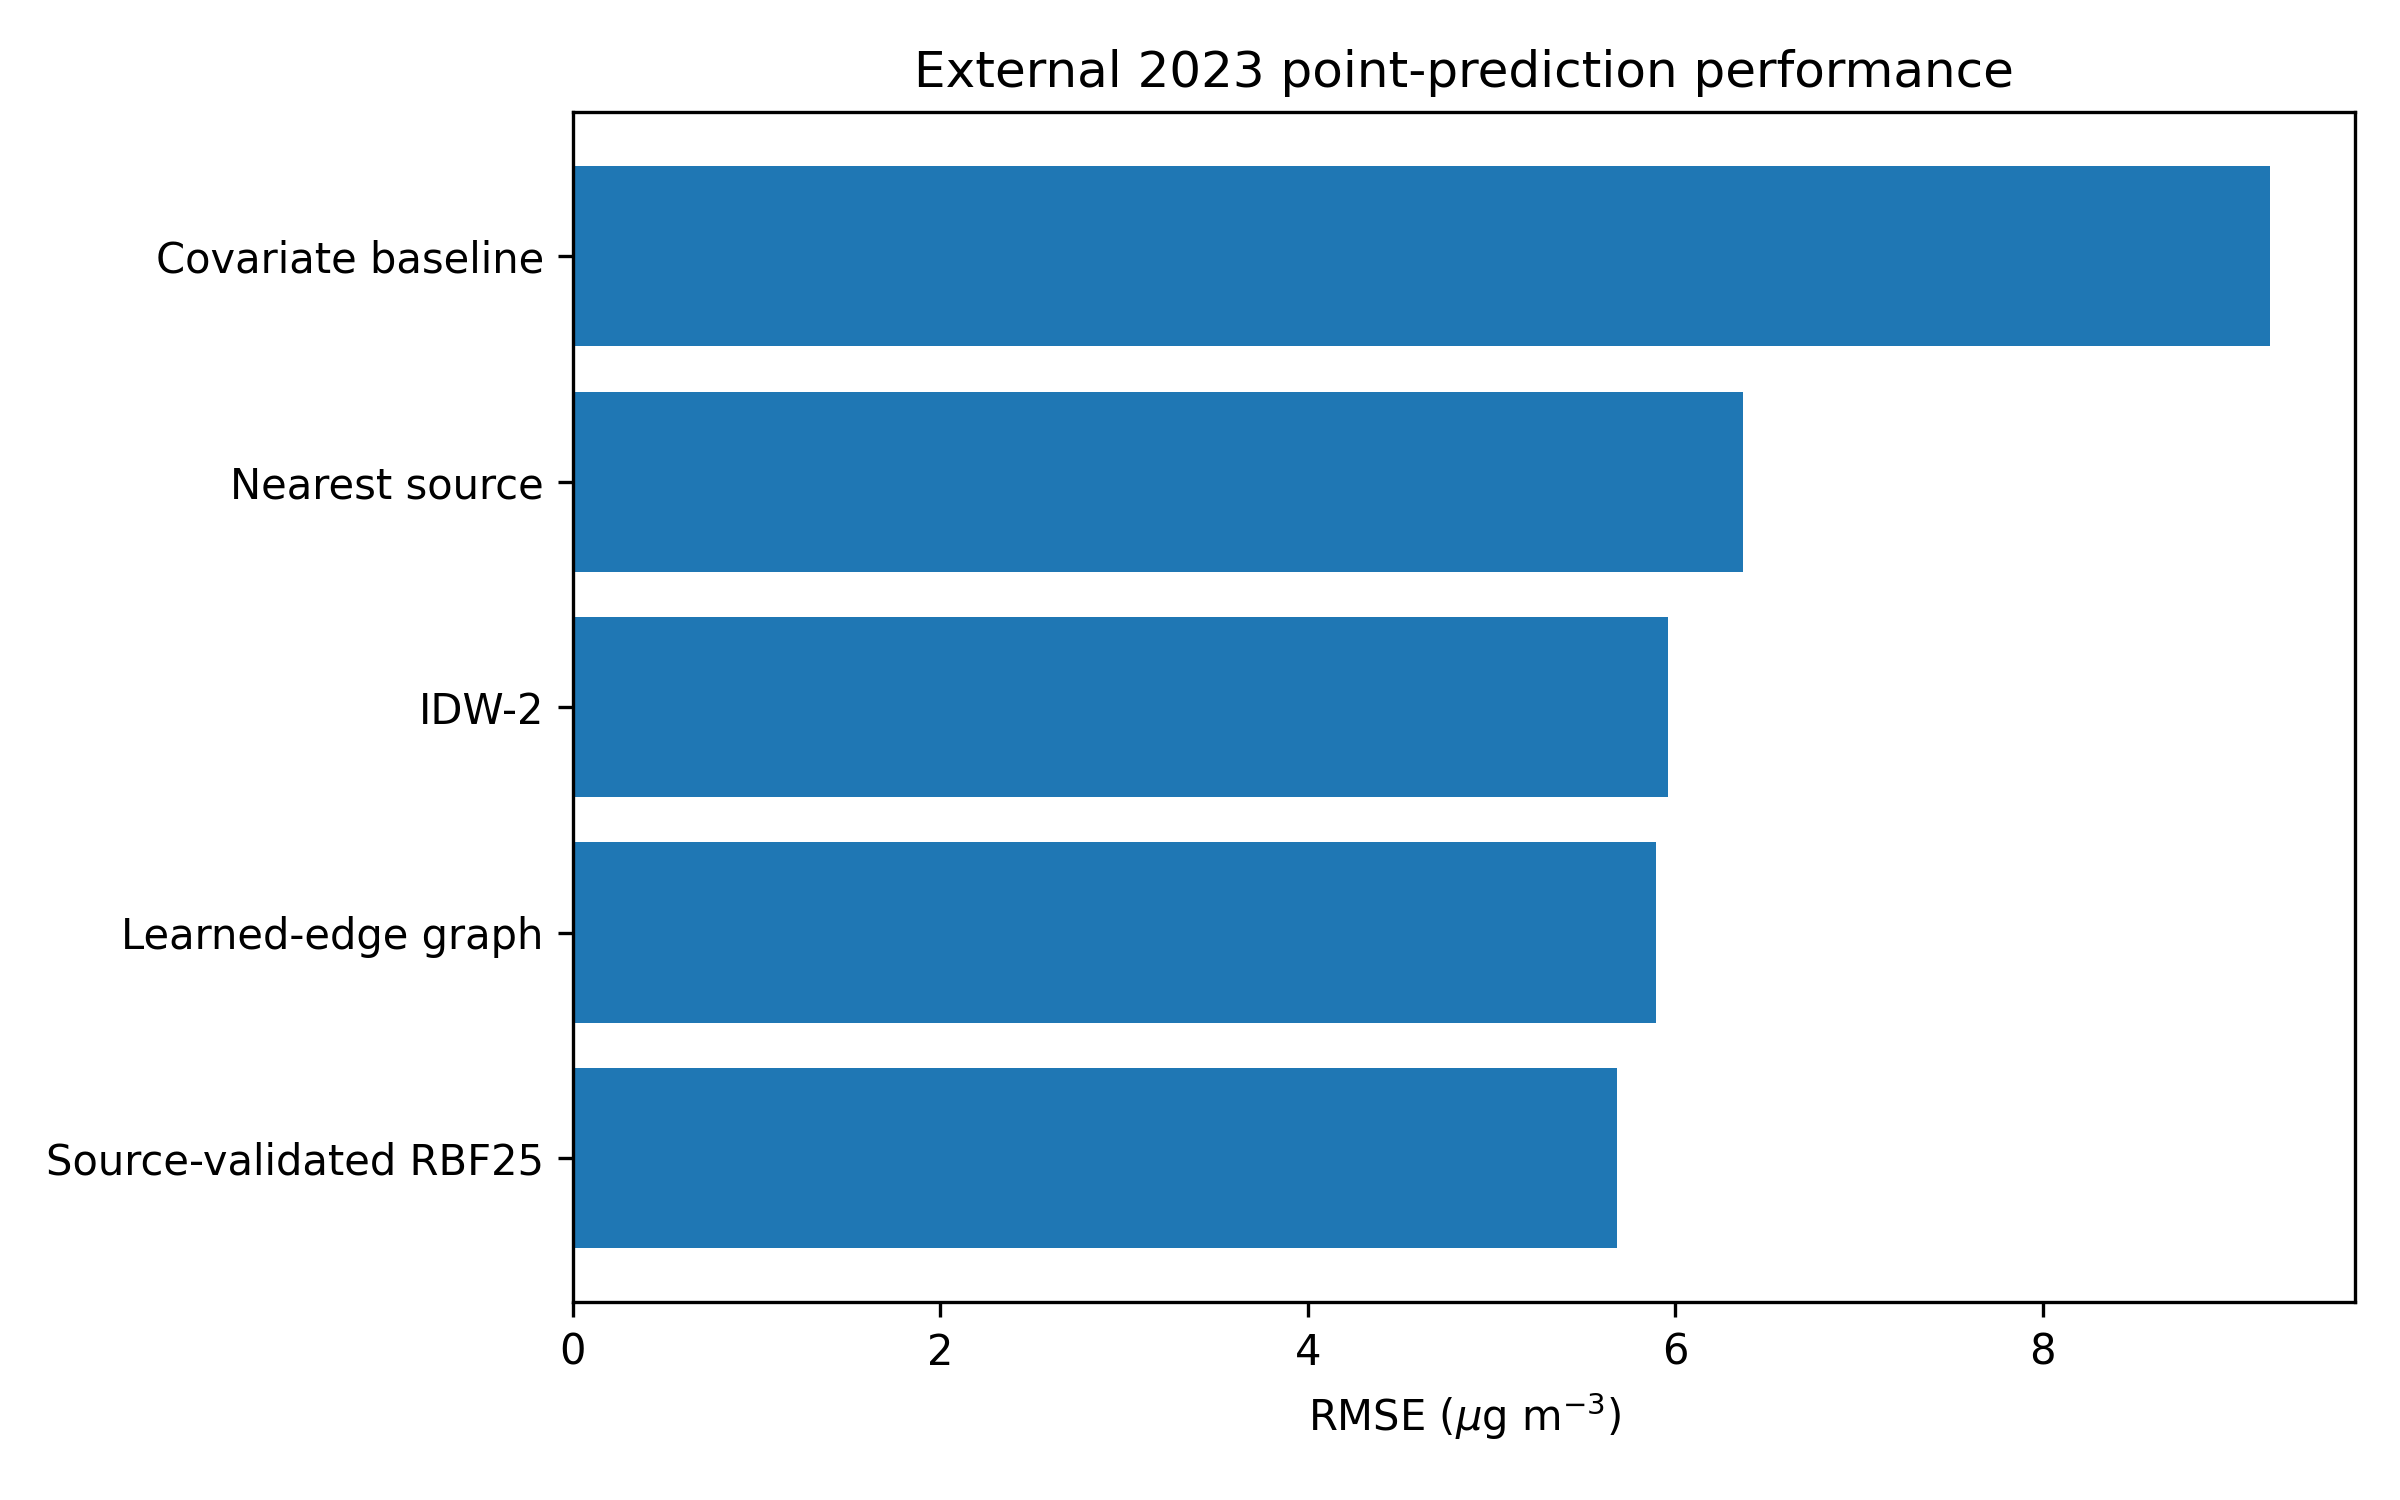
\includegraphics[width=0.82\linewidth]{figures/fig_po_final_rmse_comparison.png}
    \caption{External 2023 RMSE for the principal point-prediction methods. The simple source-validated RBF25 smoother is the strongest overall point predictor, while the learned-edge model substantially improves on the nonspatial and nearest-station baselines.}
    \label{fig:po_final_rmse}
\end{figure}

This comparison materially changes the interpretation of the empirical findings. The learned graph clearly extracts useful same-day spatial information, because it strongly improves on the covariate-only and nearest-source models. Its added flexibility does not, however, translate into uniformly lower external loss than a well-chosen local smoother. The practical value of the graph is therefore heterogeneous and should be assessed by station, season, and pollution regime rather than inferred only from the aggregate development results.

\subsection{Spatial and seasonal heterogeneity}
\label{subsec:po_heterogeneity}

The learned graph was better than the source-validated RBF25 smoother in station-level RMSE at five of the ten locked sites. The largest graph advantages occurred at STA.IT1826A, where RMSE decreased from 6.074 to 4.625, and at STA.IT0778A, where it decreased from 4.567 to 3.881. Conversely, the RBF smoother was substantially better at STA.IT1037A and STA.IT2121A. At STA.IT2121A, the graph retained a positive bias of 5.217~$\mu\mathrm{g}\,\mathrm{m}^{-3}$, indicating that the regional residual field did not fully represent the unusually low local concentration level. These site-specific reversals explain why an aggregate improvement observed during internal station-block validation did not carry uniformly into the final network expansion setting.

\begin{figure}[htbp]
    \centering
    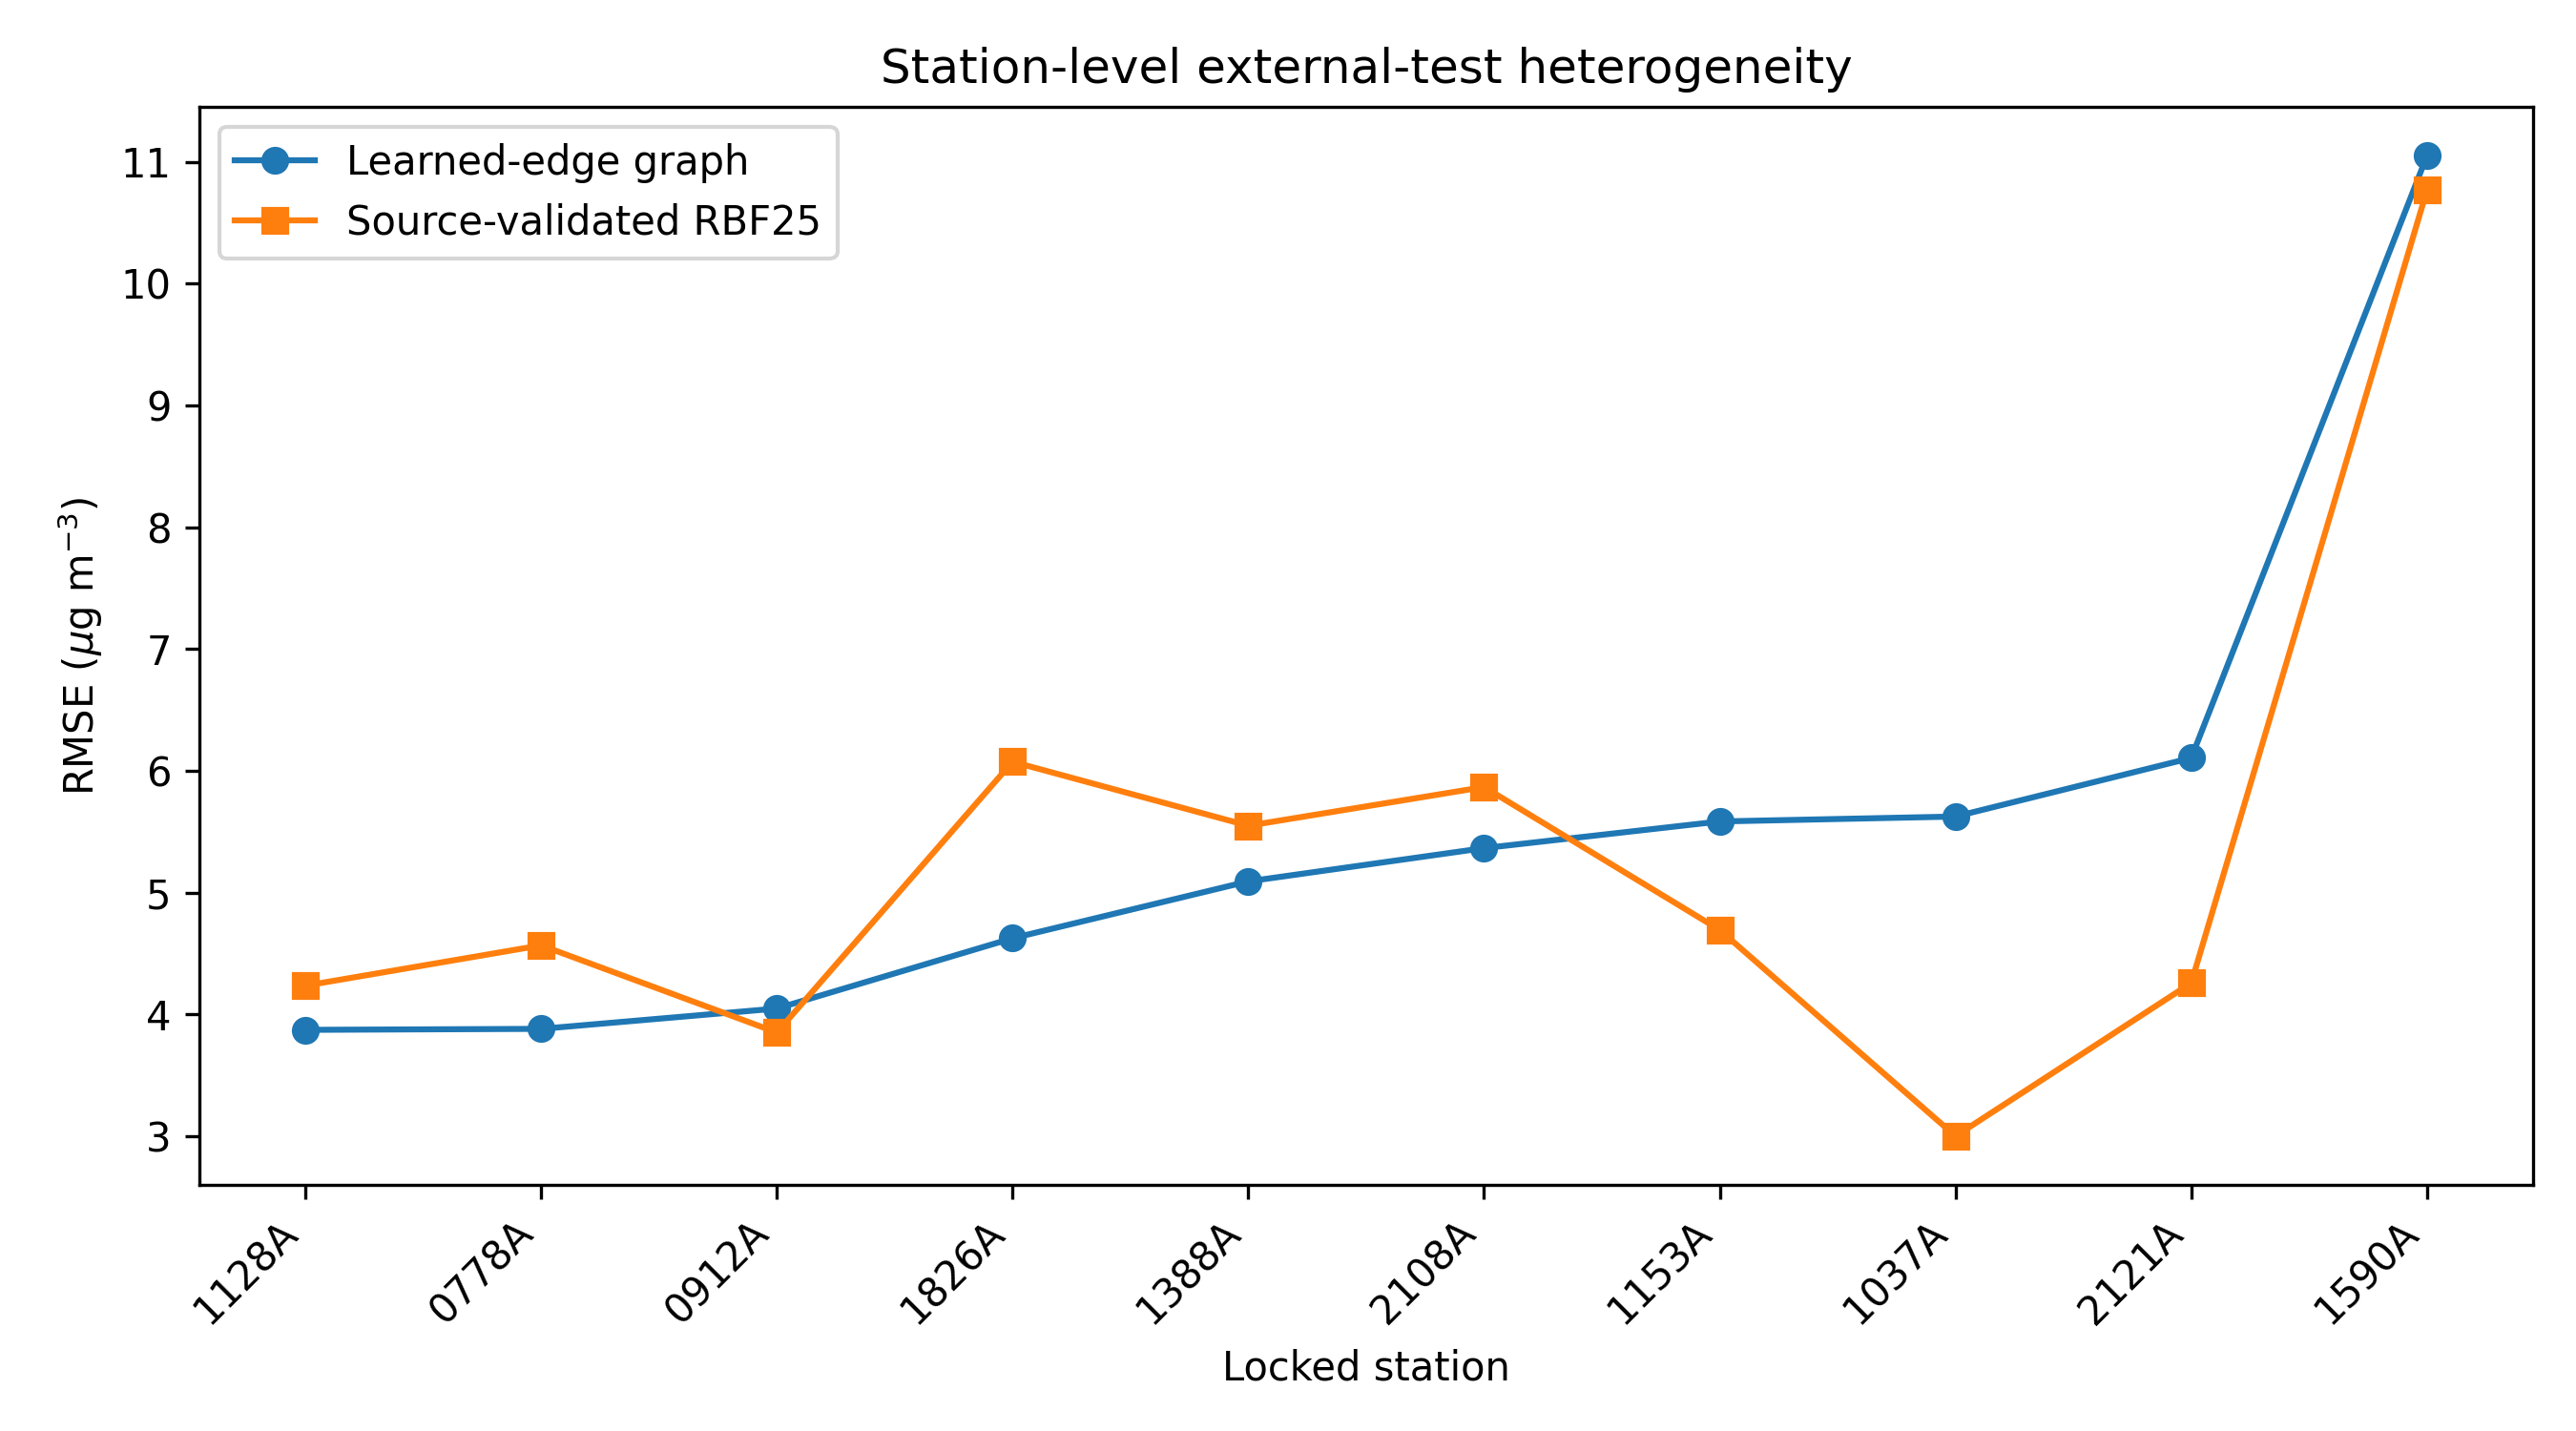
\includegraphics[width=0.90\linewidth]{figures/fig_po_station_rmse_comparison.png}
    \caption{Station-level RMSE for the learned-edge graph and the source-validated RBF25 smoother. Performance is heterogeneous: each method is superior at five of the ten locked sites.}
    \label{fig:po_station_rmse}
\end{figure}

Seasonal results are reported in Table~\ref{tab:po_season}. Both models performed best in summer and worst in winter, consistent with the larger magnitude and variability of cold-season PM$_{2.5}$. For the learned graph, RMSE increased from 3.292 in summer to 9.256 in winter, while the average 90\% interval width increased from 14.78 to 26.79. The RBF smoother was more accurate in spring, summer, and autumn. Winter performance was nearly identical in RMSE, and the learned graph obtained slightly lower winter CRPS, 4.069 versus 4.090. Thus, the additional meteorological and residual-similarity structure was most competitive in the difficult cold-season regime, but it did not improve routine warm-season interpolation.

\begin{table}[htbp]
\centering
\caption{Seasonal external-test results. CRPS and interval metrics refer to the calibrated Student-$t$ distribution of the learned-edge model. The final two columns compare point accuracy with the source-validated RBF25 smoother.}
\label{tab:po_season}
\begin{tabular}{lrrrrrr}
\toprule
Season & $n$ & RMSE & MAE & CRPS & Cov90 & RBF25 RMSE \\
\midrule
Winter & 823 & 9.256 & 5.471 & 4.069 & 0.940 & 9.226 \\
Spring & 857 & 4.476 & 3.245 & 2.409 & 0.944 & 3.961 \\
Summer & 727 & 3.292 & 2.603 & 1.929 & 0.978 & 2.894 \\
Autumn & 830 & 4.528 & 3.622 & 2.629 & 0.970 & 4.243 \\
\bottomrule
\end{tabular}
\end{table}

The most variable target was STA.IT1590A, which included an isolated observed value of 203~$\mu\mathrm{g}\,\mathrm{m}^{-3}$. Its annual mean bias was only $-0.223$, but its RMSE was 11.049 because neither the regional graph nor the local smoother reproduced the isolated spike. Figure~\ref{fig:po_timeseries_1590} shows that the model tracked the broader winter episodes while substantially underestimating this single extreme. The example illustrates why robust likelihoods and event-specific evaluation are required even when average calibration appears satisfactory.

\begin{figure}[htbp]
    \centering
    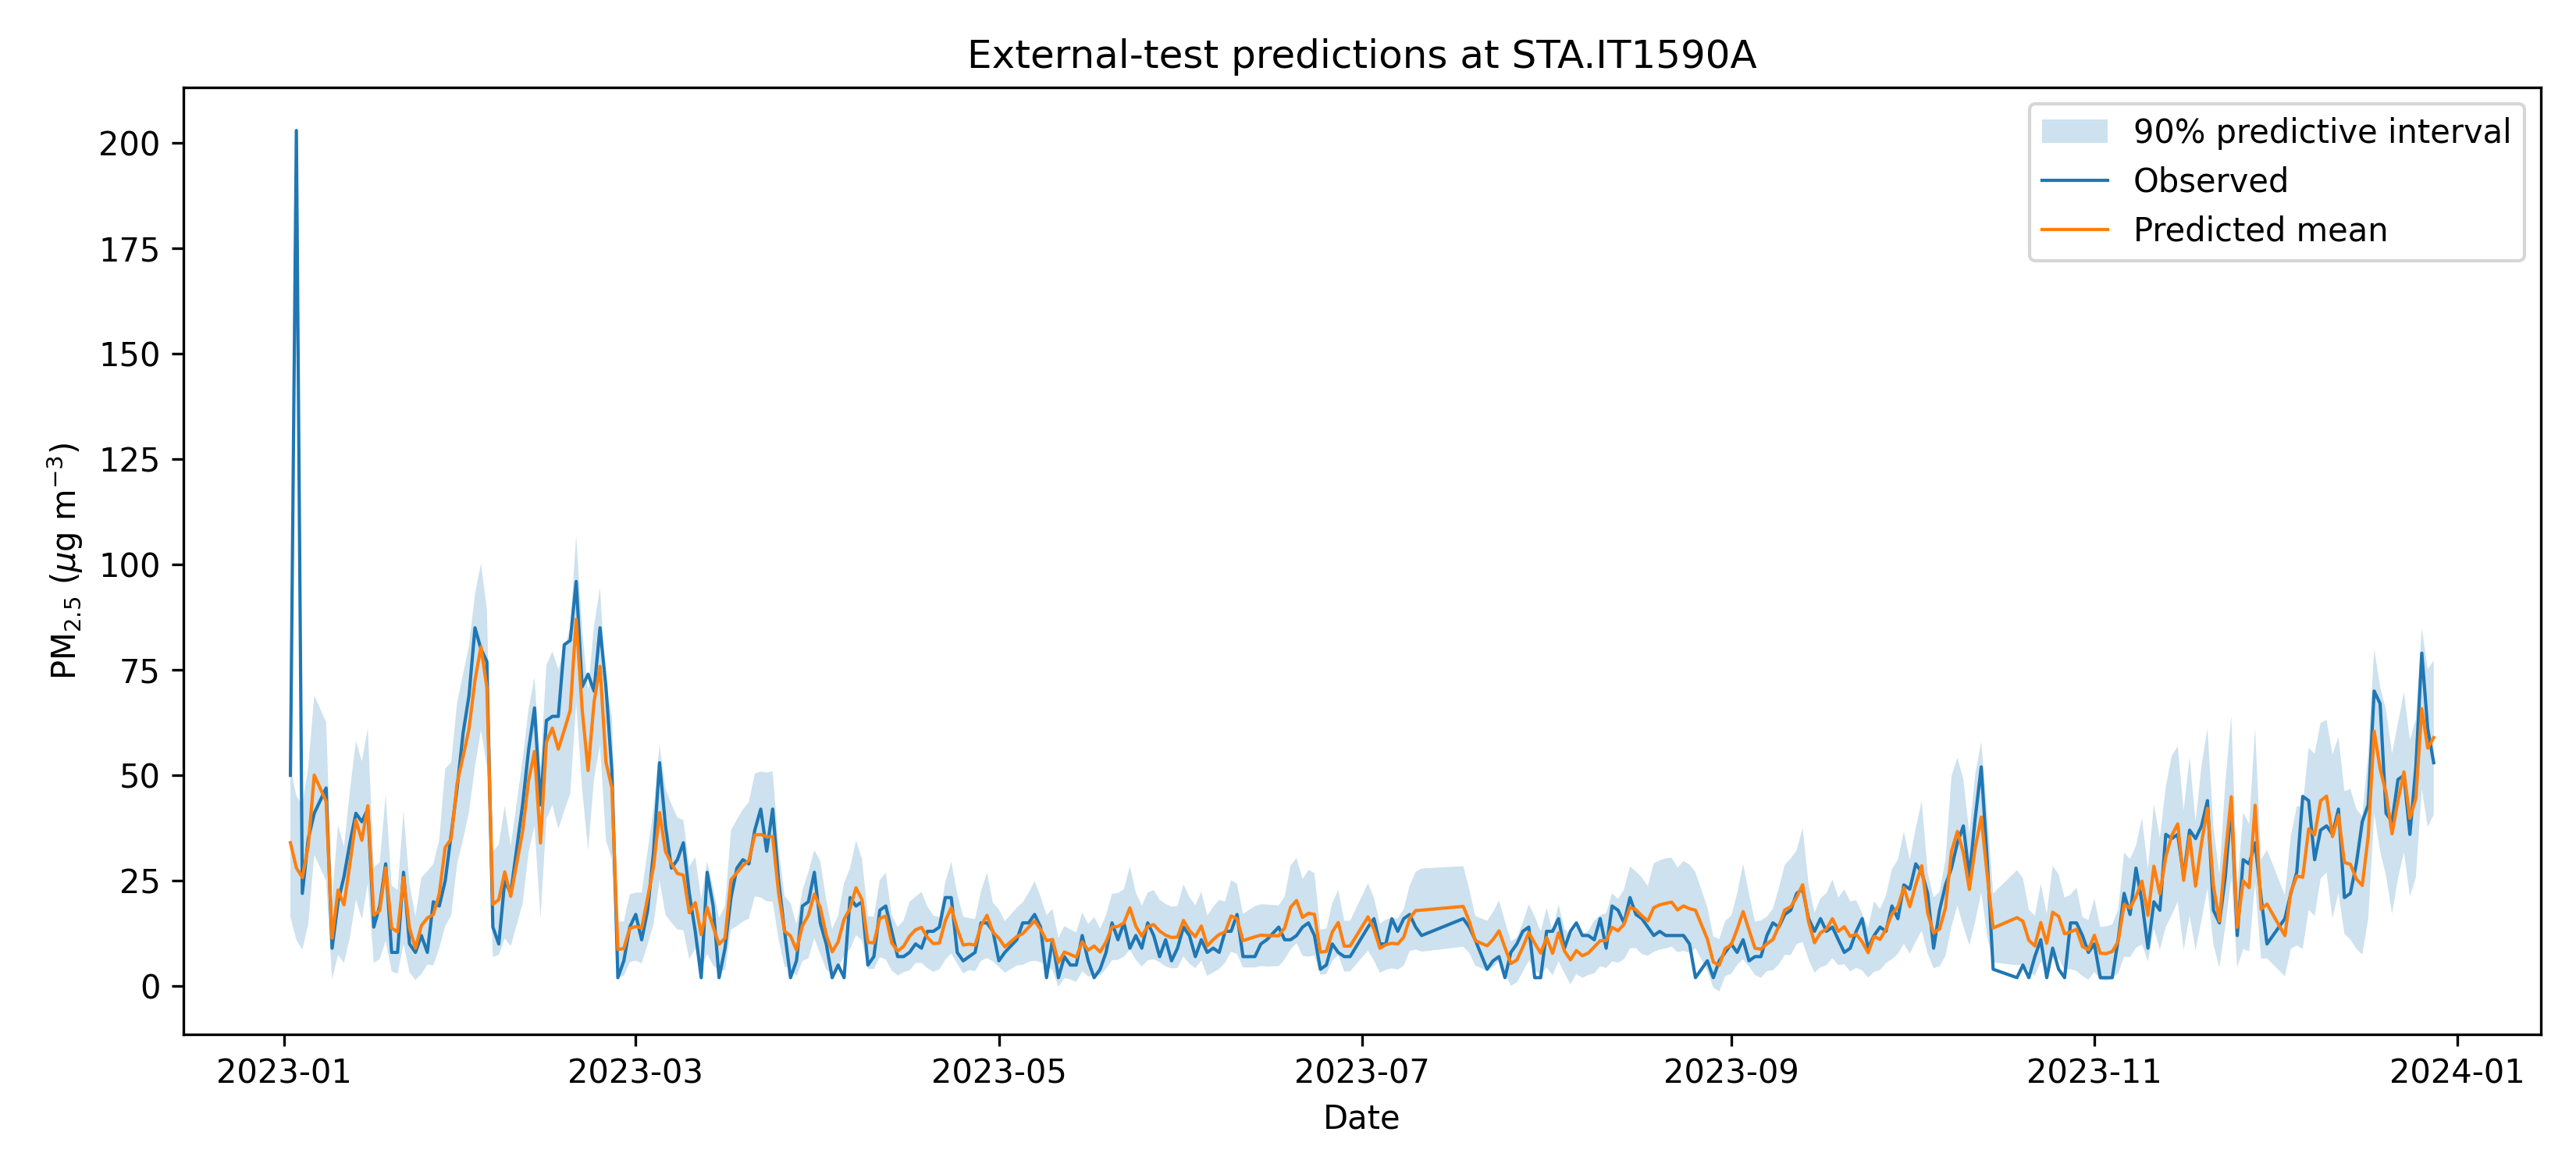
\includegraphics[width=0.96\linewidth]{figures/fig_po_timeseries_STA_IT1590A.png}
    \caption{Observed PM$_{2.5}$, learned-edge predictive mean, and calibrated 90\% interval at STA.IT1590A during 2023. The model follows the main seasonal episodes but does not reproduce the isolated value above 200~$\mu\mathrm{g}\,\mathrm{m}^{-3}$.}
    \label{fig:po_timeseries_1590}
\end{figure}

\subsection{Probabilistic calibration and high-pollution events}
\label{subsec:po_probabilistic}

The station-block conformal Student-$t$ distribution produced 90\% interval coverage of 0.957 with an average width of 19.54~$\mu\mathrm{g}\,\mathrm{m}^{-3}$. Coverage at individual sites ranged from 0.915 to 0.994. The distribution was therefore conservative on the external test, which is also visible in the reduced PIT mass near zero and one in Figure~\ref{fig:po_pit}. A mild excess of PIT values below 0.5 is consistent with the small positive mean bias of 0.435. The external overcoverage is not treated as a reason to retune the conformal factor, because the final test was opened only after the calibration rule had been frozen.

\begin{figure}[htbp]
    \centering
    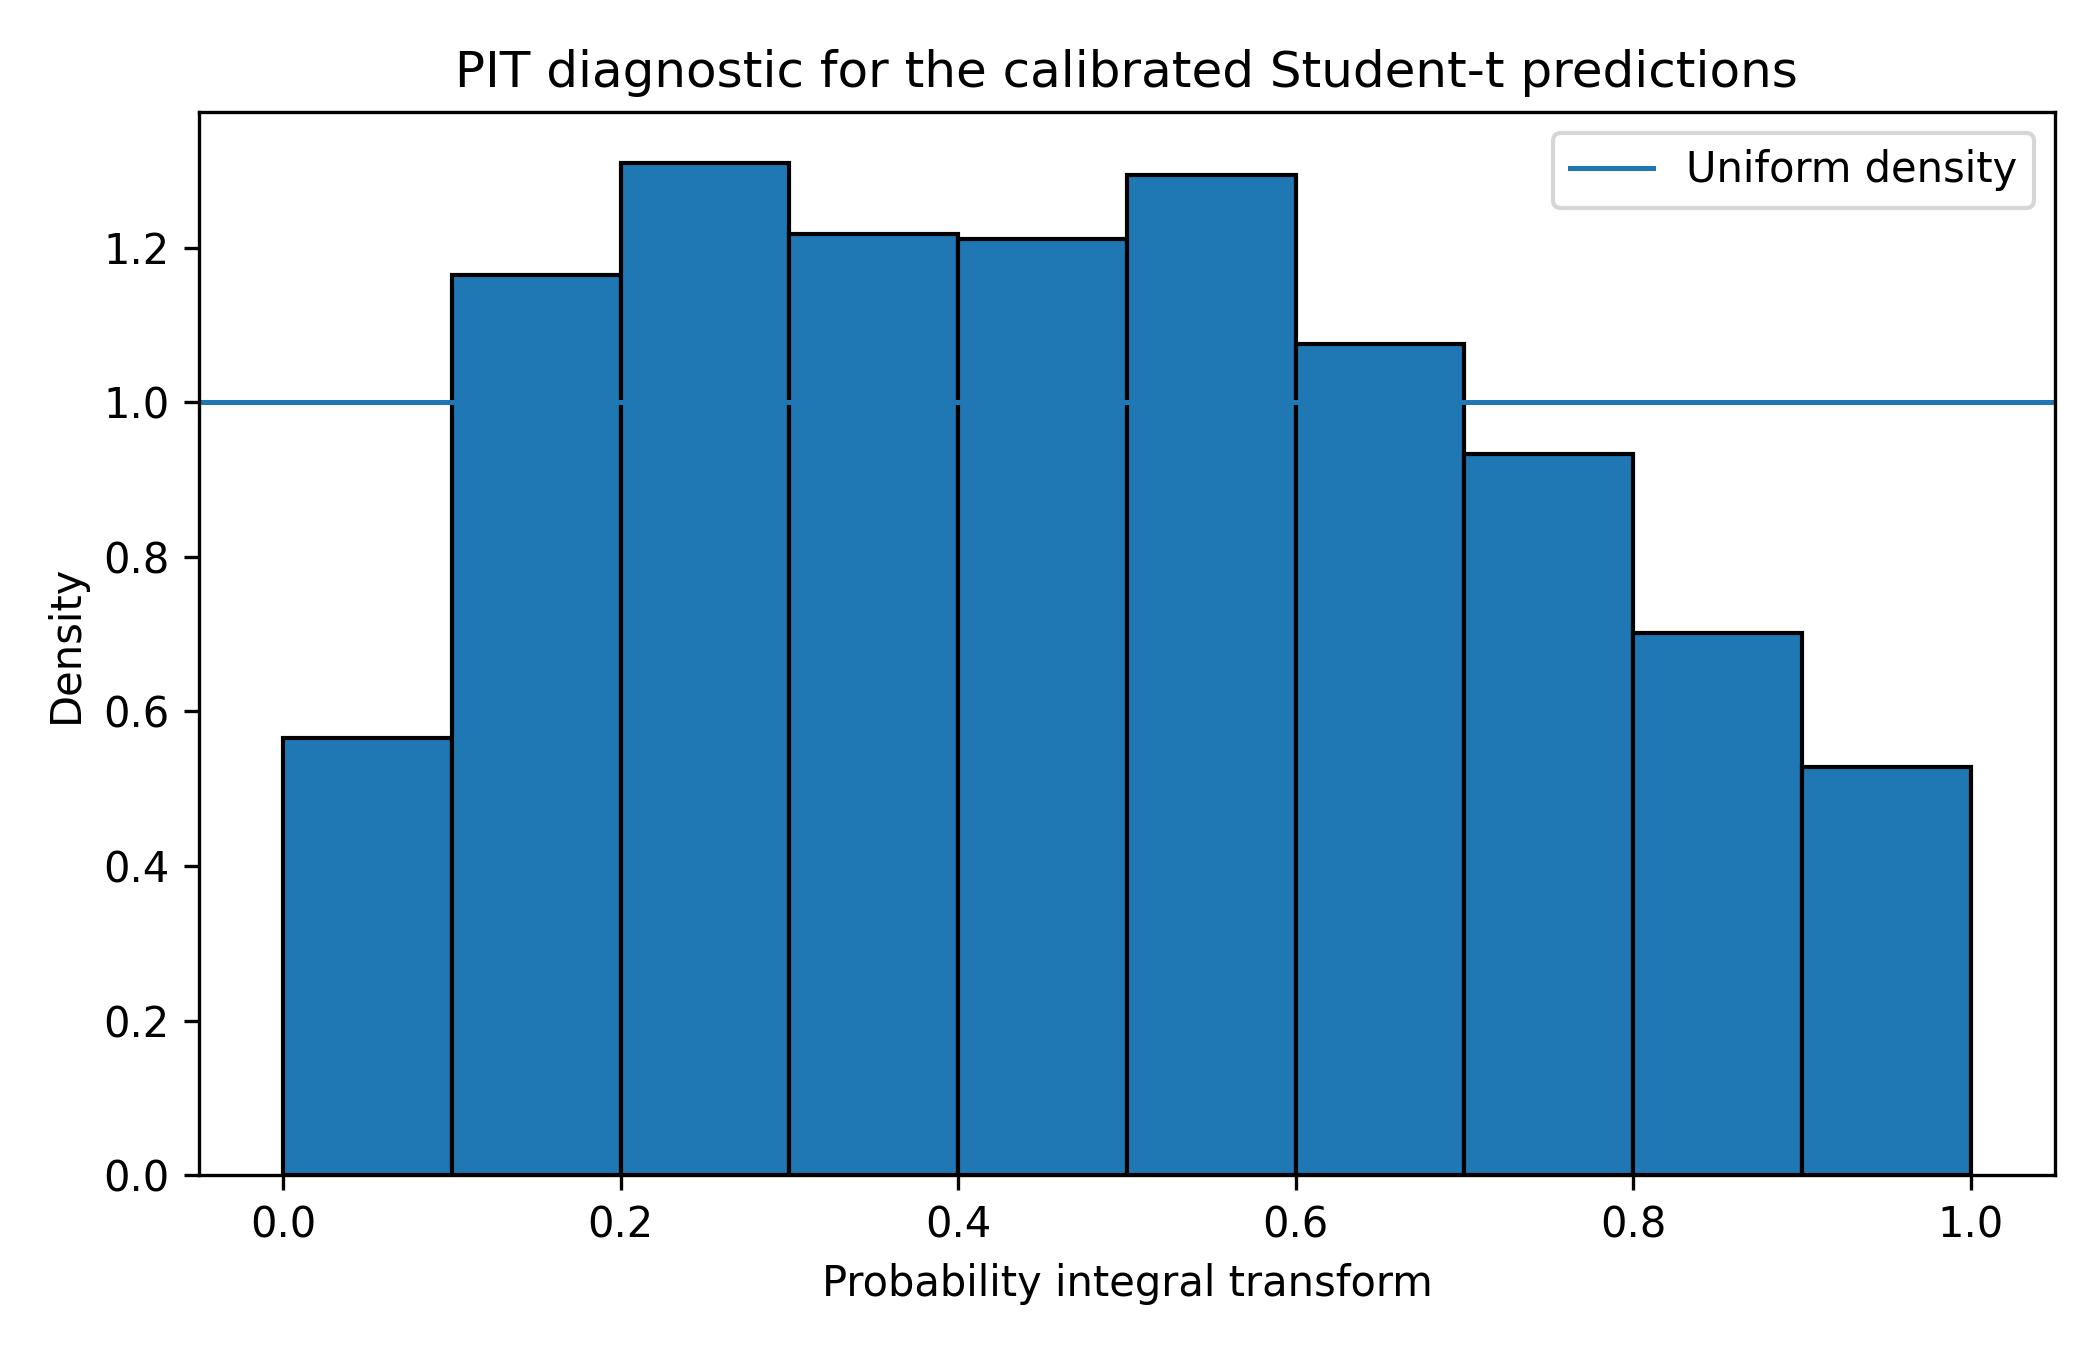
\includegraphics[width=0.76\linewidth]{figures/fig_po_pit_histogram.png}
    \caption{Probability integral transform for the locked 2023 Student-$t$ predictions. The relative shortage of values near zero and one indicates conservative predictive dispersion, while the mild leftward concentration agrees with the positive mean bias.}
    \label{fig:po_pit}
\end{figure}

Table~\ref{tab:po_final_prob} compares the learned graph with the source-validated RBF25 mean after both were equipped with the same heteroskedastic Student-$t$ and station-block conformal procedure. The RBF smoother achieved lower CRPS and log score. The paired CRPS difference, learned graph minus RBF25, was 0.198 with a 95\% daily-bootstrap interval of $[0.131,0.265]$, establishing better distributional accuracy for the simpler smoother. The learned graph produced a slightly narrower interval and a lower interval score, but the interval-score difference of $-0.496$ had a 95\% interval of $[-1.076,0.078]$ and was not conclusive.

\begin{table}[htbp]
\centering
\caption{Matched probabilistic comparison on the locked 2023 test. Both mean models use a heteroskedastic Student-$t$ scale model and station-block conformal calibration fitted without locked-station outcomes. Lower CRPS, log score, width, and interval score are better; coverage is compared with the nominal 0.90 level.}
\label{tab:po_final_prob}
\begin{tabular}{lrrrrrr}
\toprule
Mean model & CRPS & Log score & Cov90 & AIW90 & IS90 & $\nu$ \\
\midrule
Learned-edge graph & 2.780 & 2.959 & 0.957 & \textbf{19.54} & \textbf{22.52} & 12.50 \\
Source-validated RBF25 & \textbf{2.577} & \textbf{2.903} & 0.959 & 20.04 & 23.01 & 15.01 \\
\bottomrule
\end{tabular}
\end{table}

High-pollution events were defined before final evaluation by the 90th percentile of PM$_{2.5}$ in the 2018--2021 development data, equal to 39.1~$\mu\mathrm{g}\,\mathrm{m}^{-3}$. The locked test contained 205 such observations. Both probabilistic models discriminated these events well, with AUROC approximately 0.987. The learned graph had a lower Brier score, 0.0221 versus 0.0227, and a higher area under the precision--recall curve, 0.860 versus 0.843. It also had slightly lower high-event MAE, 7.960 versus 8.021, and less negative high-event bias, $-5.56$ versus $-6.03$. The RBF smoother nevertheless had lower high-event RMSE, 14.87 versus 15.52. Hence, the graph provided a small advantage in probabilistic ranking and average extreme-event error, but both methods systematically underestimated the magnitude of the most severe episodes.

\begin{table}[htbp]
\centering
\caption{Detection and prediction of high-pollution events, defined by the fixed development-period threshold of 39.1~$\mu\mathrm{g}\,\mathrm{m}^{-3}$.}
\label{tab:po_high_events}
\begin{tabular}{lrrrrrr}
\toprule
Method & Brier & AUROC & AUPRC & High RMSE & High MAE & High bias \\
\midrule
Learned-edge graph & \textbf{0.0221} & \textbf{0.9867} & \textbf{0.8598} & 15.515 & \textbf{7.960} & \textbf{$-5.563$} \\
Source-validated RBF25 & 0.0227 & 0.9867 & 0.8434 & \textbf{14.869} & 8.021 & $-6.029$ \\
\bottomrule
\end{tabular}
\end{table}

\subsection{Practical interpretation and empirical conclusion}
\label{subsec:po_interpretation}

The locked evaluation establishes three findings. First, same-day observations from the surrounding network are essential. Both spatial methods sharply improve on the meteorology-and-site-only baseline, showing that regional residual information carries substantial signal after accounting for local covariates and station climatology. Second, a strict spatial--temporal test gives a less favorable and more credible assessment than internal validation alone. The learned graph retained strong performance and useful uncertainty quantification, but its aggregate advantage over simpler spatial interpolation did not generalize. Third, the station-block conformal procedure protected coverage under spatial transfer, although it was conservative in the final year.

Operationally, the learned model is defensible when probabilistic high-event ranking, covariate-aware residual transfer, or performance at particular heterogeneous sites is important. For routine network gap filling, the source-validated 25-km RBF smoother is the stronger default because it is simpler and achieved lower RMSE, MAE, CRPS, and log score. The empirical evidence therefore does not justify presenting the learned graph as universally superior or as a replacement for classical spatial smoothing. A scientifically accurate claim is narrower: the inductive graph offers a structured, calibrated virtual-sensing mechanism that substantially improves nonspatial and nearest-source prediction, is competitive in winter and at several difficult sites, and provides modest gains for probabilistic identification of high-pollution episodes, while a carefully validated local kernel remains the strongest overall comparator.

This result also determines the appropriate scope of the manuscript. The contribution should be framed around leakage-resistant evaluation, station-block uncertainty calibration, and the conditions under which flexible graph learning does or does not improve virtual sensing. Claims of state-of-the-art point-prediction dominance would not be supported by the locked external test.
